\newpage
\section{\centering Point Spread Function}

\subsection{Définition}

La fonction d'étalement du point (= \textsl{Point Spread Function}), appelée \textbf{PSF}, est une fonction représentant la réponse d'un système optique à une source lumineuse ponctuelle. Dans notre cas, il s'agit de la réponse de l'optique de l'ELT à une étoile et son (ou ses) exoplanète(s).

Elle dépend de la longueur d'onde de la lumière observée, de la qualité de l'optique, de la turbulence atmosphérique, de la position de l'objet observé, etc... Pour la calculer, on calcule la transformée de Fourier en deux dimensions de la pupille de l'instrument. % * C'est pas la TF d'une source ponctuelle de 2D plutôt ? je comprends pas trop :/

\subsection{La PSF de la pupille de L’ELT}

Prenons l'exemple de la PSF d'une étoile à travers la pupille de l'ELT. En calculant la PSF d'une étoile à travers cette pupille, on obtient une forme particulière, qui dépend de la longueur d'onde observée.

\begin{figure}[htbp]
\centering
\begin{subfigure}[b]{0.40\textwidth}
\centering

\includegraphics[width=\textwidth]{figures/ELT_pupil.png}
\caption{Pupille de l'ELT. on peut voir les 6 araignées de l'ELT permettant de soutenir le miroir secondaire ainsi que le miroir secondaire y sont représenté. La partie blanche représentente les zones laissant passer la lumières.}
\label{fig:elt_pupil}
\end{subfigure}
\hfill
\begin{subfigure}[b]{0.46\textwidth}
\centering
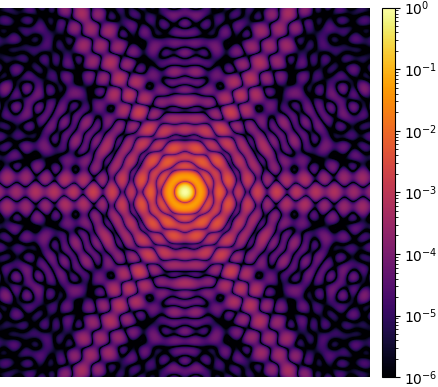
\includegraphics[width=\textwidth]{figures/PSF_ELT.png}
\caption{PSF normalisé de l'ELT représenté en échelle logarithme.}
\label{fig:pupil_diff}
\end{subfigure}
\caption{\textit{None}}
\end{figure}

On normalise la PSF pour que l'intensité lumineuse soit égale à 1 en son centre, et qu'on puisse voir l'image sous forme de contraste. Cela permet de mieux visualiser les zones où une exoplanète d'un certain contraste comparé à l'étoile serait potentiellement visible.

Dans la figure \ref{fig:pupil_diff}, on peut voir que l'on n'obtient pas exactement une fonction de Bessel d'ordre 1, mais une forme similaire avec un pic central et des anneaux de diffraction autour. Cette différence de forme est lié aux araignées de l'ELT et au miroir central qui viennent perturber la propagation de la lumière.

\begin{figure}[htbp]
\centering
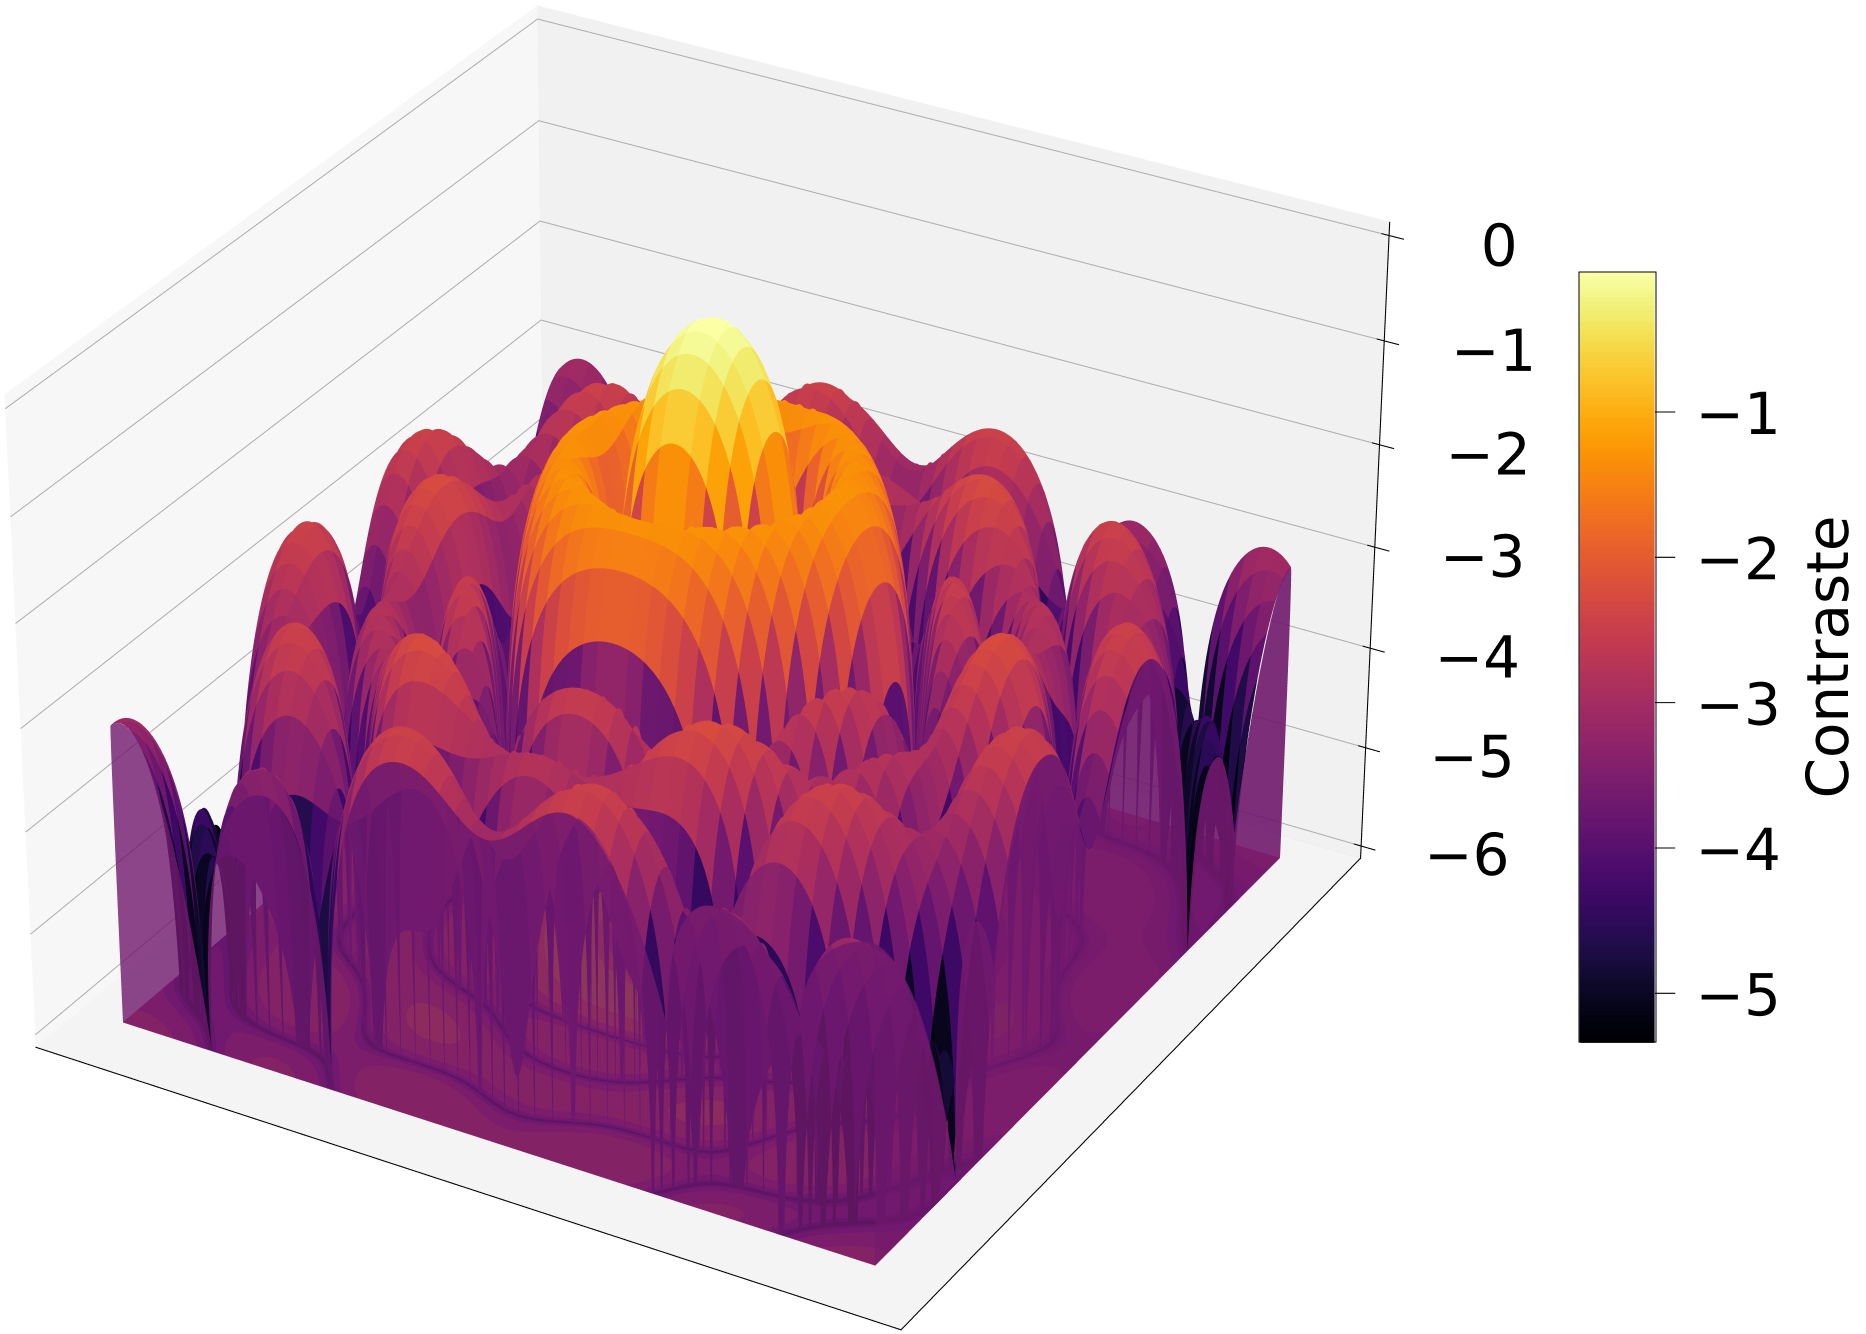
\includegraphics[width=0.7\textwidth]{figures/PSF_ELT_3D_bord.png}
\caption{Représentation 3D de la PSF normalisé de l'ELT représenté en échelle logarithme. On peut voir les anneaux de diffraction autour du pic central.}
\label{fig:3D_PSF}
\end{figure}


La représentation 3D de la PSF zoomée en échelle logarithme dans la figure \ref{fig:3D_PSF} permet de mieux se rendre compte des anneaux de diffraction, et des reliefs de contraste dans la PSF lié à la diffraction.

On se rend donc compte assez facilement de la difficulté de détecter la présence d'une exoplanète à faible séparation d'une étoile, car la PSF de l'étoile est bien trop intense comparé au contraste de l'exoplanète, qui sera trop faible en comparaison.


% comment on le calcule dans le code

\subsection{Exemple avec un apodiseur d'HARMONI}

Afin de visualiser les effets d'un apodiseur, nous pouvons nous reférer 
aux deux apodiseurs prévues pour le HCM : l'apodiseur SP1 \ref{fig:SP1}, dont l'objectif et de créer une zone de haut contraste proche de l'étoile, et l'apodiseur SP2 \ref{fig:SP2}, qui a pour but d'observer une zone beaucoup plus large mais moins proche de l'étoile. L'avantage de ces deux apodiseurs est qu'ils permettent à eux seuls l'observation d'un vaste champ de vue, permettant d'observer différents objets potentiellement présents autour d'étoiles. À 1.45 µm, SP1 permet d'observer de 42 mas à 89 mas, et SP2 de 57 mas à 295 mas, et pourront atteindre un contraste de $10^{-6}$.

On peut voir que les zones de hauts contrastes sont net et défini par 2 rayons limites : l'Inner Working Angle (IWA) et l'Outer Working Angle (OWA). Ces deux angles correspondent à la séparation angulaire minimum et maximum imposé dans lequel on souhaite créer la zone de haut contraste.
% In the latter case, the result is that planets with a flux ratio of 10−6 may be detected as close as 50mas from the star, and with a flux ratio of a few 10−7 at 100mas.
%A constraint was in fact set on the relative intensity of that light in a region than encompasses the whole FoV, so that this its mean value would not be higher than the maximum intensity of the AO halo in the high-contrast region, which may be as low as 10−4 in good seeing conditions (first quartile, 0.43”).
% * Les contrastes atteints par chacun ?

% ! An exploration of the parameter space (minimum and maximum separations, contrast, and throughput) concluded that a 35% throughput could be achieved while satisfying the robustness, contrast, and maximum separation requirements if the minimum separation was set to 7.3λ/D. By comparison, satisfying them for a 6λ/D minimum separation would result in a twice as low throughput. A 7.3λ/D minimum separation corresponds to a 96mas angular distance on sky, which satisfies the top-level requirement of HARMONI.

%The HCM is designed to observe in the H and K bands. Since the PSF scales with the wavelength, it is necessary to use two FPM for each apodizer, unless the minimum separation of one in the H band corresponds to the minimum separation of the other in the K band, in which case only three FPM are required in total, and this solution was chosen given the limited number of available FPM.

On remarque que l'apodiseur SP2 à l'air plus fragmenté comparé au SP1; cela est du à la différence de fréquence spatiale apodisé : plus on cherche à créer une zone de haut contraste éloigné du centre, plus les fréquence spatiale à diffracté seront ??? et plus l'apodiseur sera 'fragmenté'. % * je sais plus exactement comment ça marche :p

\begin{figure}[htbp]
\centering
% Première ligne avec SP1
\begin{subfigure}[b]{0.40\textwidth}
\centering
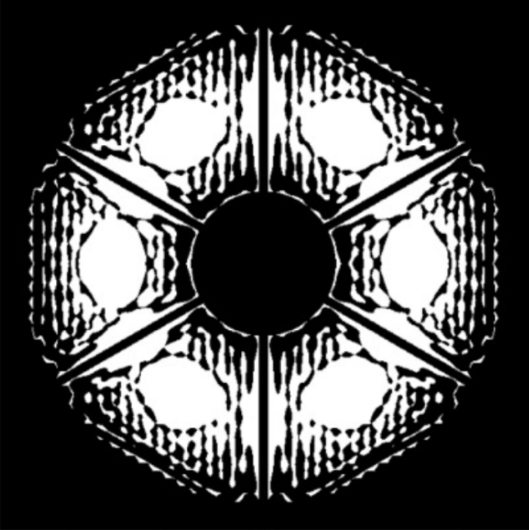
\includegraphics[width=\textwidth]{figures/SP1_HARMONI.png}
\caption{Apodiseur SP1 de HARMONI-ELT.}
\label{fig:SP1}
\end{subfigure}
\hfill % Espace entre les images
\begin{subfigure}[b]{0.45\textwidth}
\centering
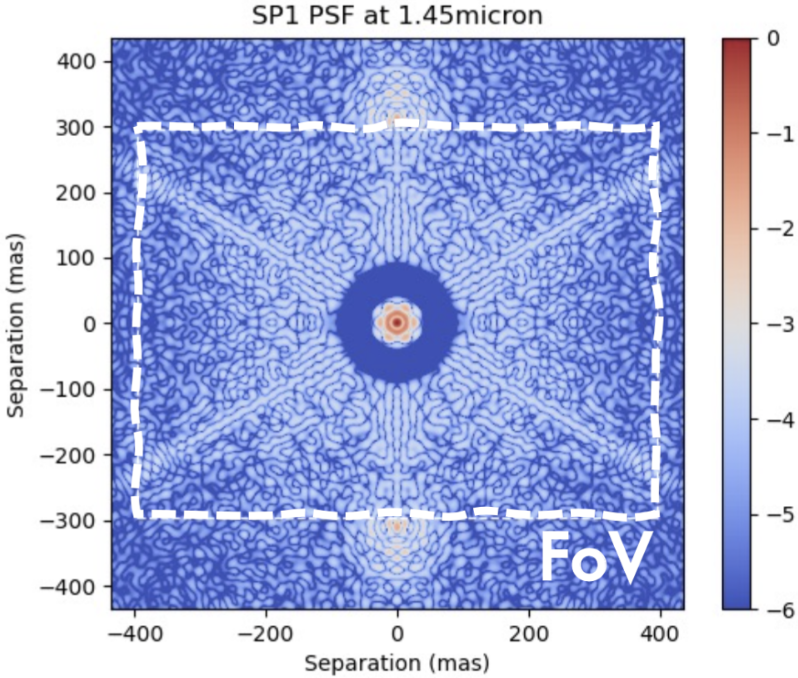
\includegraphics[width=\textwidth]{figures/PSF_SP1_HARMONI.png}
\caption{PSF SP1 de HARMONI-ELT.}
\label{fig:PSF_SP1}
\end{subfigure}
% Deuxième ligne avec SP2
\begin{subfigure}[b]{0.40\textwidth}
    \centering
    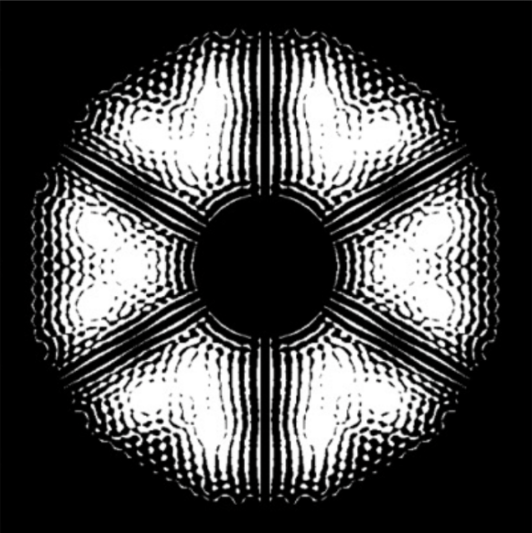
\includegraphics[width=\textwidth]{figures/SP2_HARMONI.png}
    \caption{Apodiseur SP2 de HARMONI-ELT.}
    \label{fig:SP2}
\end{subfigure}
\hfill % Espace entre les images
\begin{subfigure}[b]{0.45\textwidth}
    \centering
    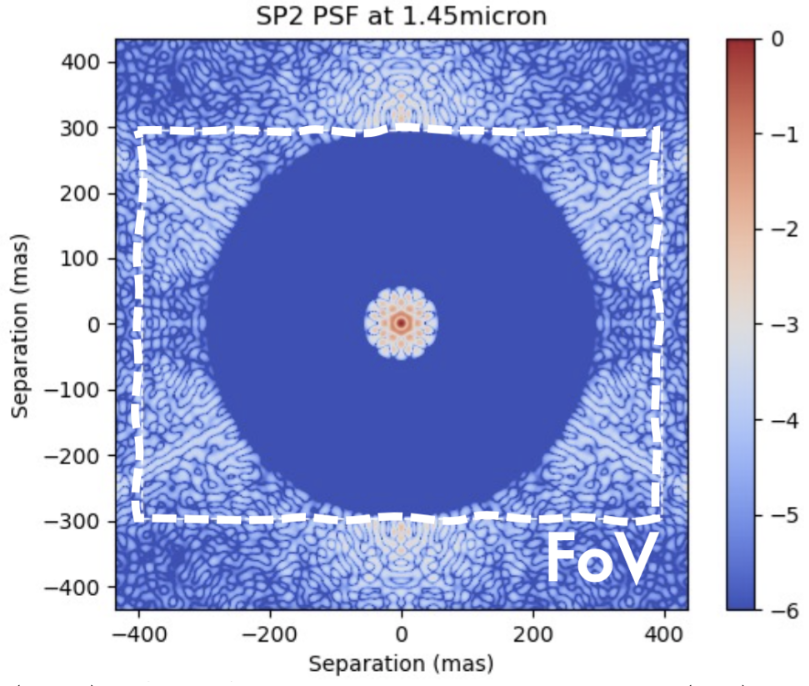
\includegraphics[width=\textwidth]{figures/PSF_SP2_HARMONI.png}
    \caption{PSF SP2 de HARMONI-ELT.}
    \label{fig:PSF_SP2}
\end{subfigure}

\caption{\textit{Comparaison des apodiseurs et des PSF pour SP1 et SP2 de HARMONI-ELT.}}
\end{figure}

\subsection{Nyquist}

On rappelle la définition de la fréquence de Nyquist : c'est la fréquence maximale que l'on peut observer dans un signal échantillonné. Elle est égale à la moitié de la fréquence d'échantillonnage.

Dans notre cas, cela signifie que pour observer correctement une planète, il faut que la planète soit échantillonnée par au moins 2 pixels par $\lambda/D$.

On présente 3 cas :

- On se trouve en dessous de Nyquist

Pas assez de données, on peut pas correctement analyser les données et affirmer ce qu'on voit (planète ou pas)

- On se trouve au dessus de Nyquist, on peut voir la planète
au moins 2 pixels par lambda/D
- On se trouve au dessus de Nyquist
temps de calcul trop long
- On se trouve à Nyquist

on peut voir la planète et analyser les données sans que ça prenne trop de temps de calcul
